%----------------------------------------------------------------------------------------
%
% LaTeX-template for degree projects at LNU, Department of Computer Science
% Last updated by Johan Hagelbäck, Oct 2015
% Linnaeus University
%
% License: Creative Commons BY
%
%----------------------------------------------------------------------------------------

%----------------------------------------------------------------------------------------
%	Settings and configuration
%----------------------------------------------------------------------------------------

\documentclass[a4paper,12pt]{article}
\usepackage[T1]{fontenc}
\usepackage{times}
\usepackage[english]{babel}
\usepackage[utf8]{inputenc}
\usepackage{caption}
\usepackage{subcaption}
\usepackage{wallpaper}
\usepackage[absolute]{textpos}
\usepackage[top=2cm, bottom=2.5cm, left=3cm, right=3cm]{geometry}
\usepackage{appendix}
\usepackage[nottoc]{tocbibind}
\usepackage[hidelinks]{hyperref}
\setcounter{figure}{0}
%\setcounter{secnumdepth}{3}
%\setcounter{tocdepth}{3}
\usepackage{amsmath}
\numberwithin{figure}{section}
\usepackage{sectsty}
\sectionfont{\fontsize{14}{15}\selectfont}
\subsectionfont{\fontsize{12}{15}\selectfont}
\subsubsectionfont{\fontsize{12}{15}\selectfont}

\usepackage{csquotes} % Used to handle citations

\renewcommand{\thetable}{\arabic{section}.\arabic{table}}  
\renewcommand{\thefigure}{\arabic{section}.\arabic{figure}} 

%----------------------------------------------------------------------------------------
%	
%----------------------------------------------------------------------------------------
\newsavebox{\mybox}
\newlength{\mydepth}
\newlength{\myheight}

\newenvironment{sidebar}%
{\begin{lrbox}{\mybox}\begin{minipage}{\textwidth}}%
{\end{minipage}\end{lrbox}%
 \settodepth{\mydepth}{\usebox{\mybox}}%
 \settoheight{\myheight}{\usebox{\mybox}}%
 \addtolength{\myheight}{\mydepth}%
 \noindent\makebox[0pt]{\hspace{-20pt}\rule[-\mydepth]{1pt}{\myheight}}%
 \usebox{\mybox}}

%----------------------------------------------------------------------------------------
%	Title section
%----------------------------------------------------------------------------------------
\newcommand\BackgroundPic{
    \put(-2,-3){
    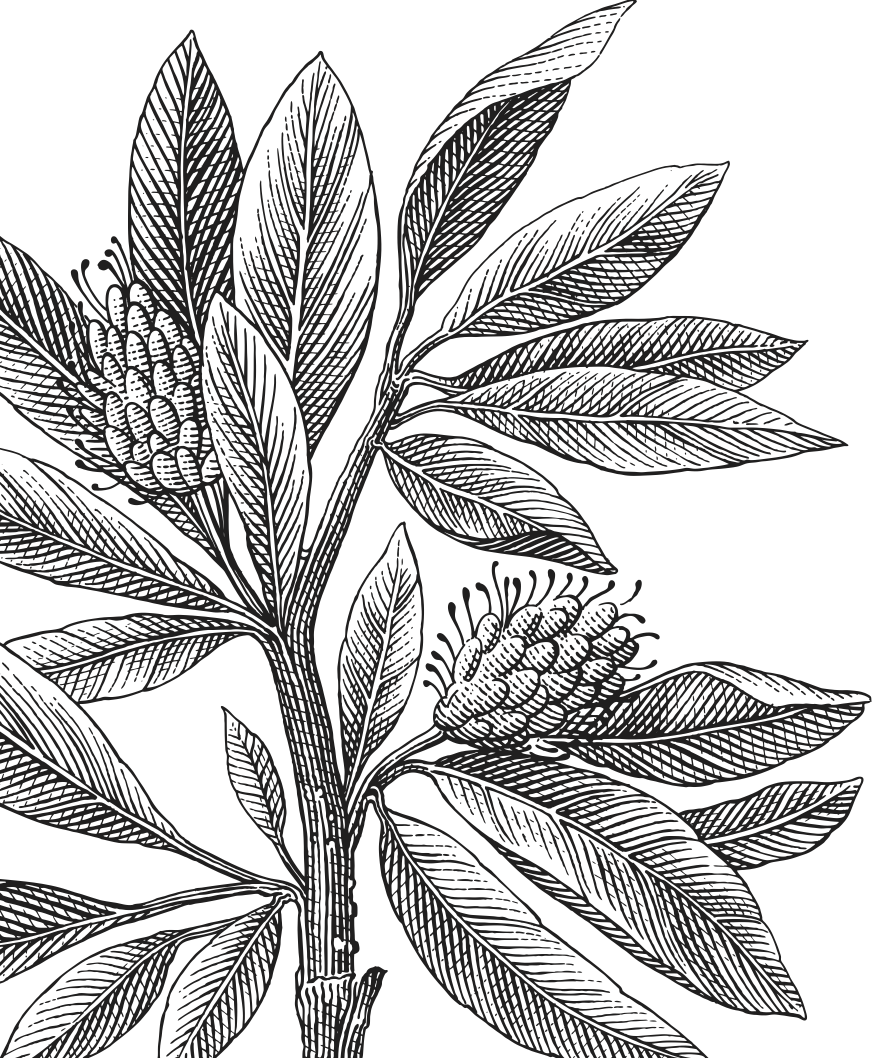
\includegraphics[keepaspectratio,scale=0.3]{img/lnu_etch.png} % Background picture
    }
}
\newcommand\BackgroundPicLogo{
    \put(30,740){
    
\includegraphics[keepaspectratio,scale=0.10]{img/logo.png} % Logo in upper left corner
    }
}

\title{	
\vspace{-8cm}
\begin{sidebar}
    \vspace{10cm}
    \normalfont \normalsize
    %\Huge Bachelor/Master Thesis Project \\
    \vspace{-1.3cm}
\end{sidebar}
\vspace{3cm}
\begin{flushleft}
    \huge Computer networks - 1DV701 \\ 
    \LARGE  Assignment 2\\
\end{flushleft}
\null
\vfill
\begin{textblock}{6}(10,13)
\begin{flushright}
\begin{minipage}{\textwidth}
\begin{flushleft} \large
\emph{Author:} Michael Johansson \& Jacob Heyder\\ % Author
%\emph{Supervisor:} Name of your supervisor\\ % Supervisor
%\emph{Examiner:} Dr.~Mark \textsc{Brown}\\ % Examiner (course manager)
\emph{Semester:} VT 2017\\ % 
%\emph{Subject:} Computer Science\\ % Subject area
\end{flushleft}
\end{minipage}
\end{flushright}
\end{textblock}
}

\date{} 

\begin{document}
\pagenumbering{gobble}
\newgeometry{left=5cm}
\AddToShipoutPicture*{\BackgroundPic}
\AddToShipoutPicture*{\BackgroundPicLogo}
\maketitle
\restoregeometry
\clearpage


%----------------------------------------------------------------------------------------
\newpage
\pagenumbering{gobble}
\tableofcontents % Table of contents
\newpage
\pagenumbering{arabic}

%----------------------------------------------------------------------------------------
%
%	Here follows the actual text contents of the report.
%
%----------------------------------------------------------------------------------------

\section{Assignment summary}

\section{Problem one}

We choose to create an Index file every time an user requests a directory. This way we have index links to the files in that directory to help with the navigation and it looks good. But if the user ask for a file/directory that doesn't exist on the server we send back a 404(File not found).We also link to our secret folder in this main index but if we click on it we get an 403 (access denied).
 
\begin{figure}[h!]
	\centering
	\label{Directory}
	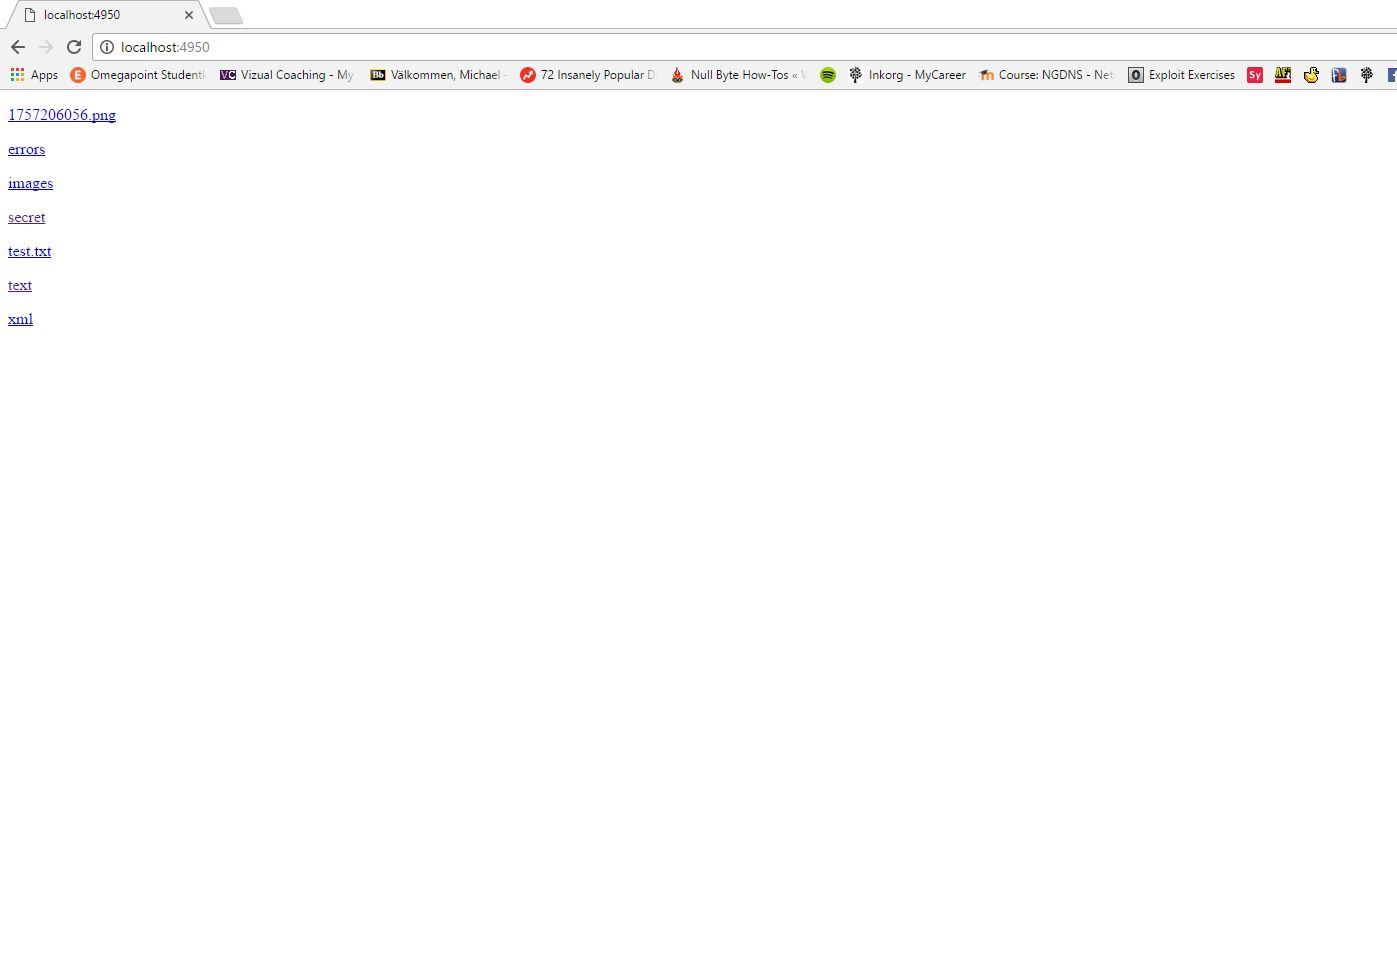
\includegraphics[width=0.95\textwidth,keepaspectratio]{img/Directory.jpg} 
	\caption{GET request on a directory, responds with index.html}
\end{figure}

\begin{figure}[h!]
	\centering
	\label{HTML}
	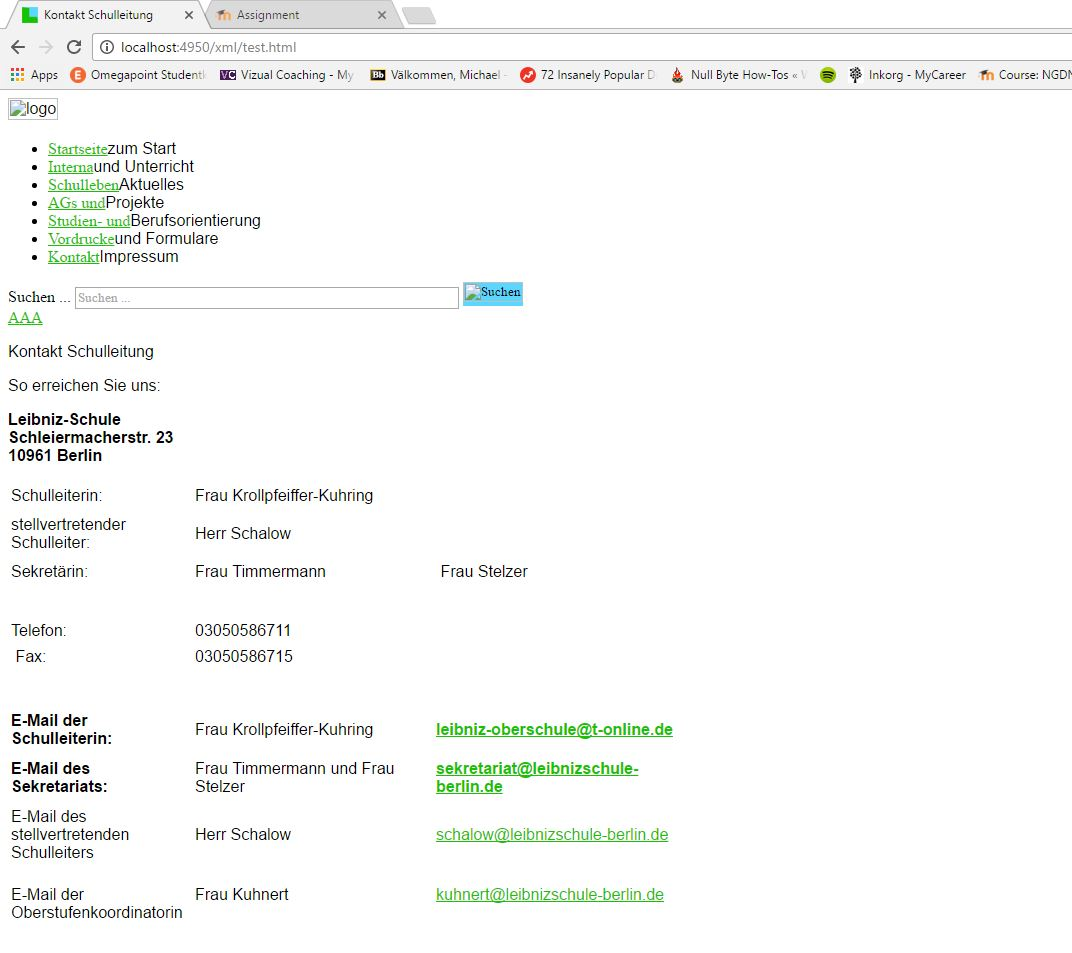
\includegraphics[width=0.95\textwidth,keepaspectratio]{img/HTMLFile.jpg} 
	\caption{GET request on a HTML file}
\end{figure}

\begin{figure}[h!]
	\centering
	\label{image}
	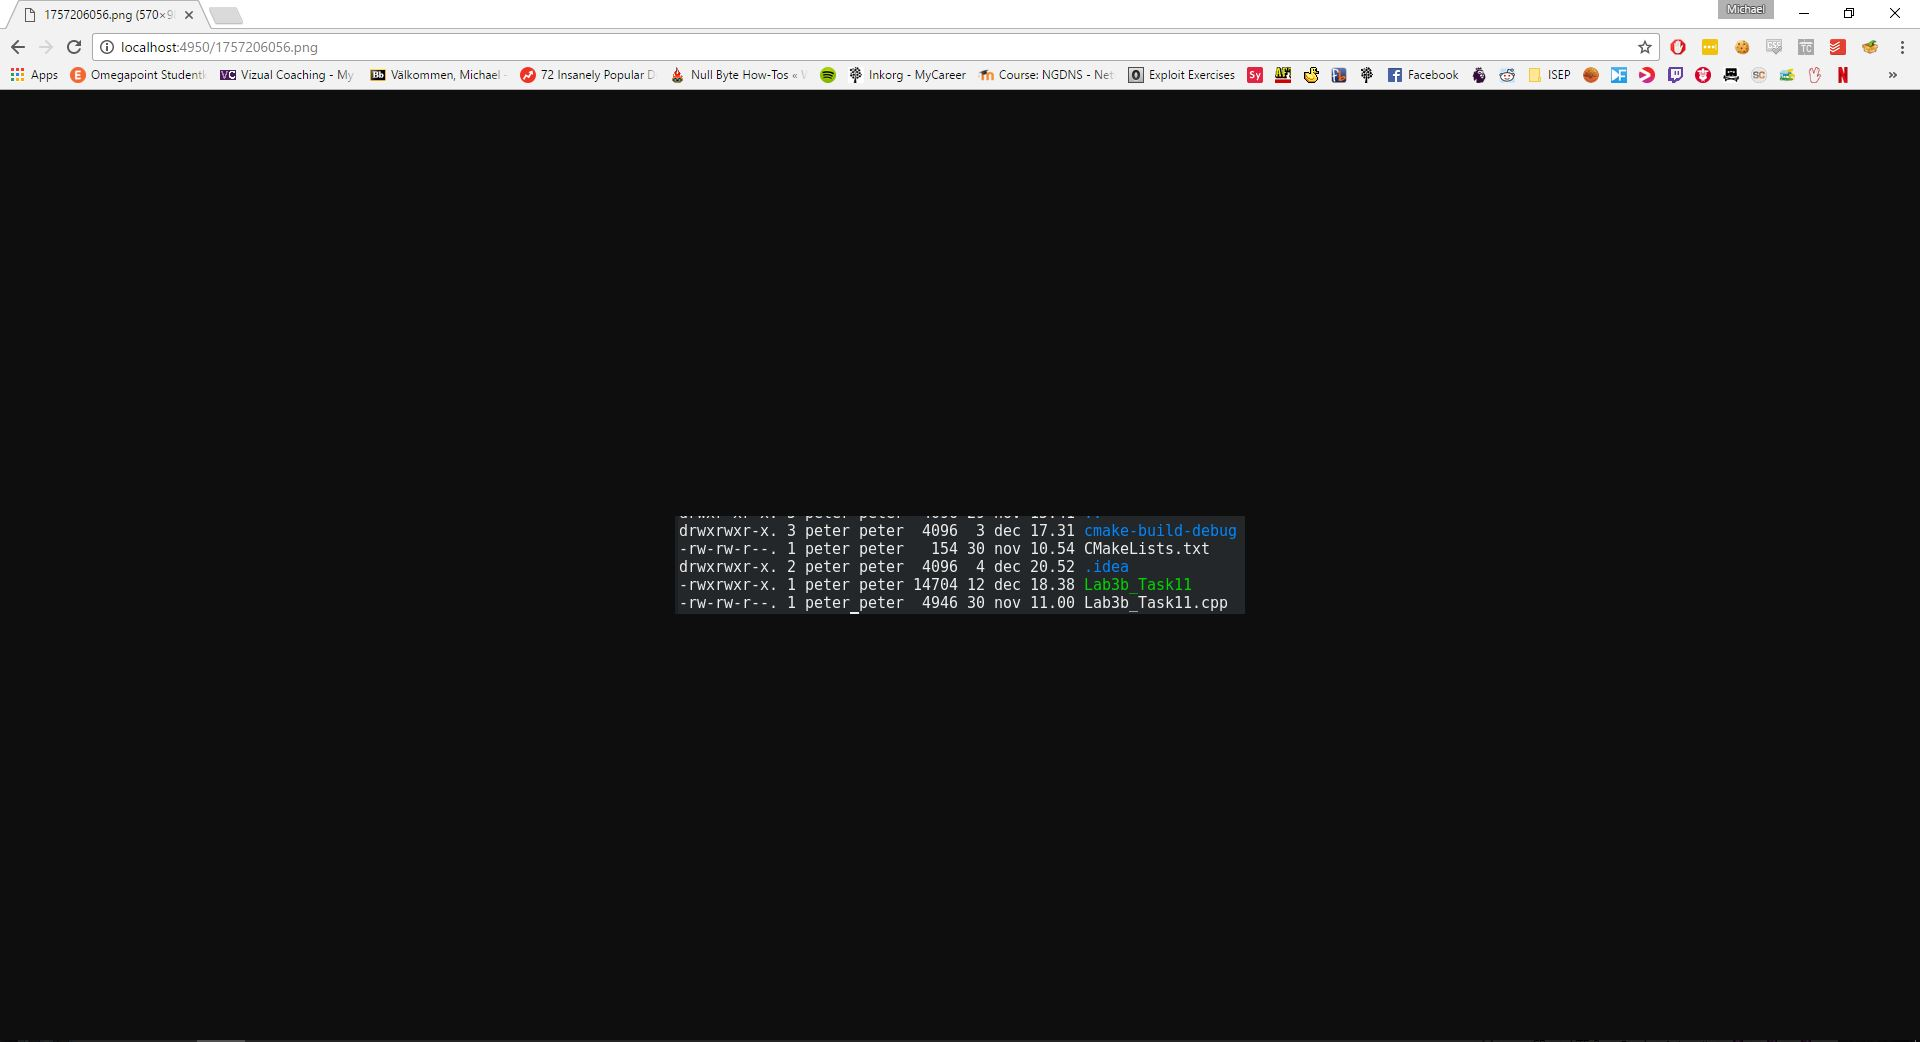
\includegraphics[width=0.95\textwidth,keepaspectratio]{img/PNGFile.jpg} 
	\caption{GET request on an image}
\end{figure}

\newpage

\section{Problem two}

\begin{figure}[h!]
	\centering
	\label{Access denied}
	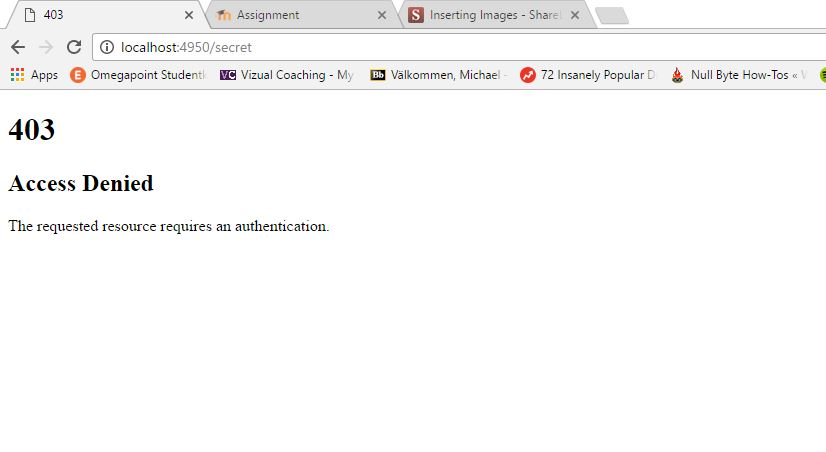
\includegraphics[width=0.95\textwidth,keepaspectratio]{img/403.jpg} 
	\caption{403 Access denied when trying to access our secret folder}
\end{figure}

\begin{figure}[h!]
	\centering
	\label{not found}
	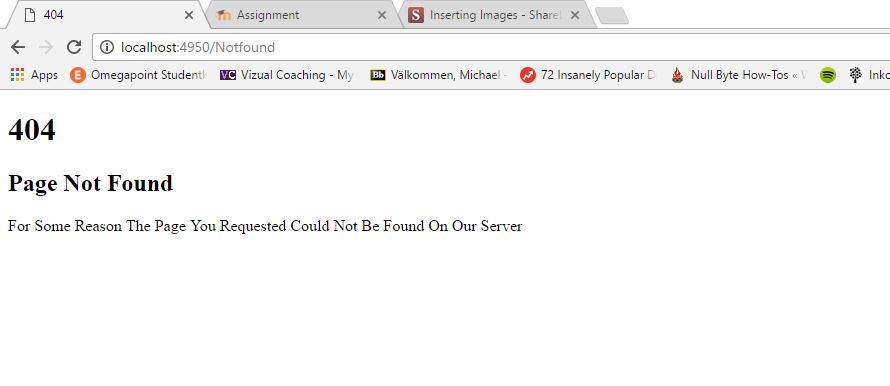
\includegraphics[width=0.95\textwidth,keepaspectratio]{img/404.jpg} 
	\caption{404 Not Found when trying to GET a resource that don't exist on the server}
\end{figure}

\begin{figure}[h!]
	\centering
	\label{Server error}
	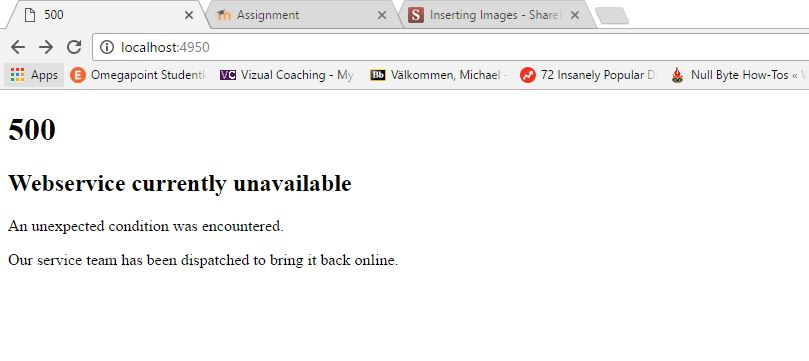
\includegraphics[width=0.95\textwidth,keepaspectratio]{img/500.jpg} 
	\caption{500 for any internal server errors, socket error etc.}
\end{figure}

\subsection{VG.1}

\begin{figure}[h!]
	\centering
	\label{201}
	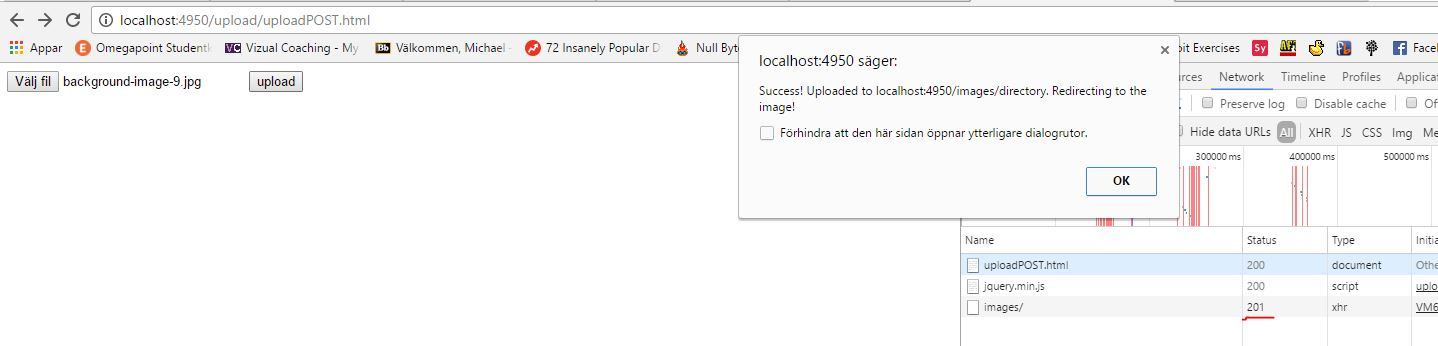
\includegraphics[width=0.95\textwidth,keepaspectratio]{img/201.jpg} 
	\caption{500 for any internal server errors, socket error etc.}
\end{figure}

\begin{figure}[h!]
	\centering
	\label{204}
	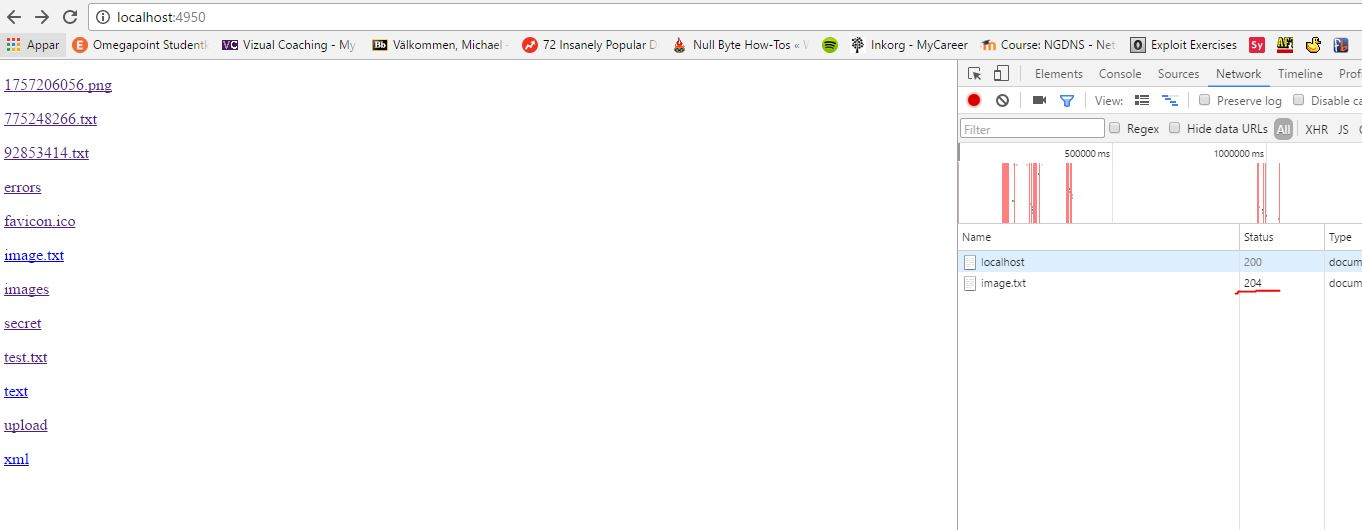
\includegraphics[width=0.95\textwidth,keepaspectratio]{img/204.jpg} 
	\caption{500 for any internal server errors, socket error etc.}
\end{figure}

\begin{figure}[h!]
	\centering
	\label{302}
	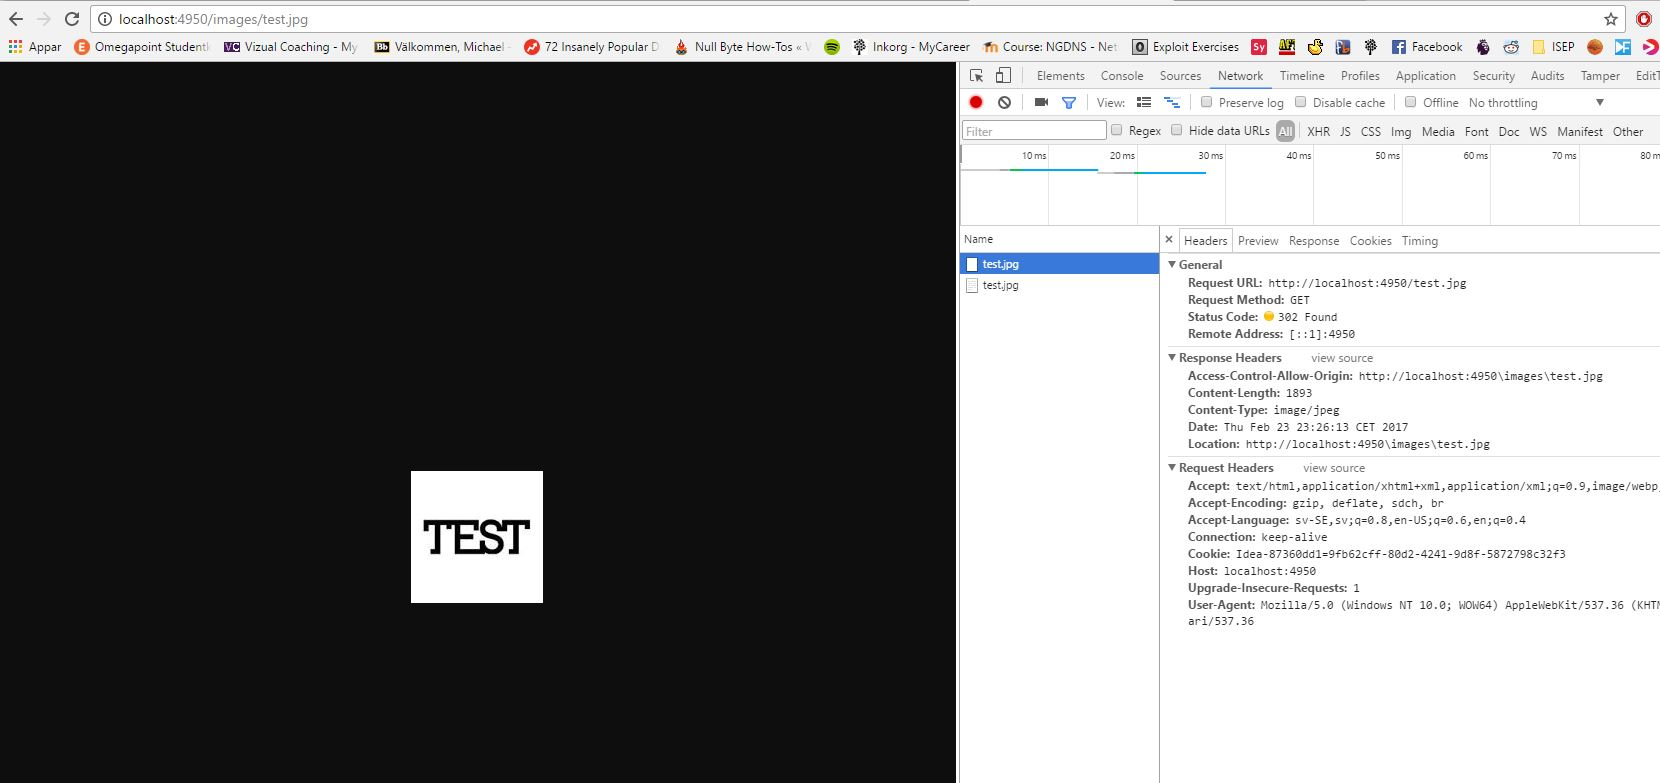
\includegraphics[width=0.95\textwidth,keepaspectratio]{img/302.jpg} 
	\caption{500 for any internal server errors, socket error etc.}
\end{figure}

\begin{figure}[h!]
	\centering
	\label{411}
	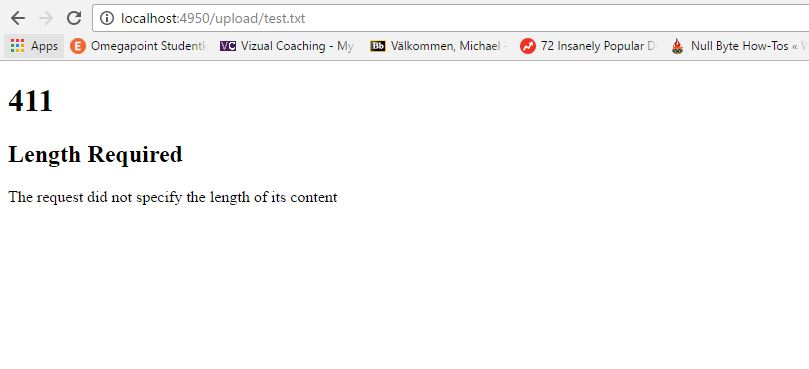
\includegraphics[width=0.95\textwidth,keepaspectratio]{img/411.jpg} 
	\caption{500 for any internal server errors, socket error etc.}
\end{figure}

\begin{figure}[h!]
	\centering
	\label{414}
	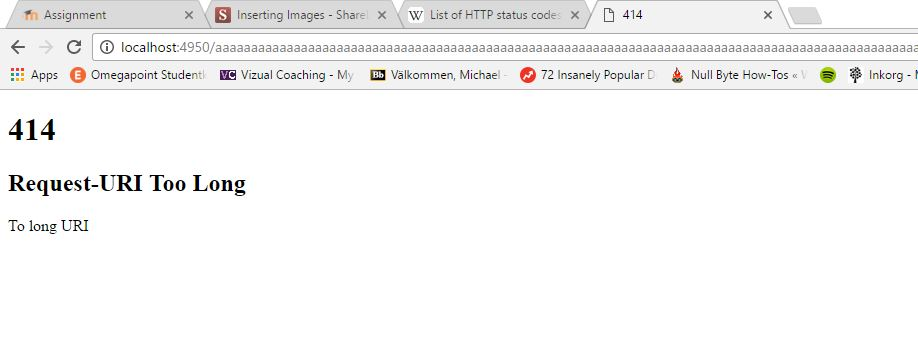
\includegraphics[width=0.95\textwidth,keepaspectratio]{img/414.jpg} 
	\caption{500 for any internal server errors, socket error etc.}
\end{figure}

\begin{figure}[h!]
	\centering
	\label{415}
	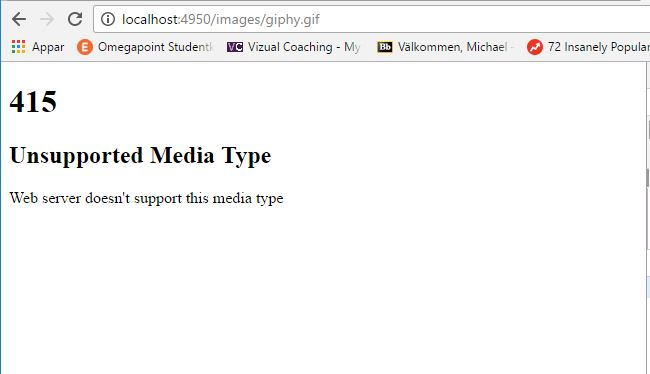
\includegraphics[width=0.95\textwidth,keepaspectratio]{img/415.jpg} 
	\caption{500 for any internal server errors, socket error etc.}
\end{figure}

\begin{figure}[h!]
	\centering
	\label{501}
	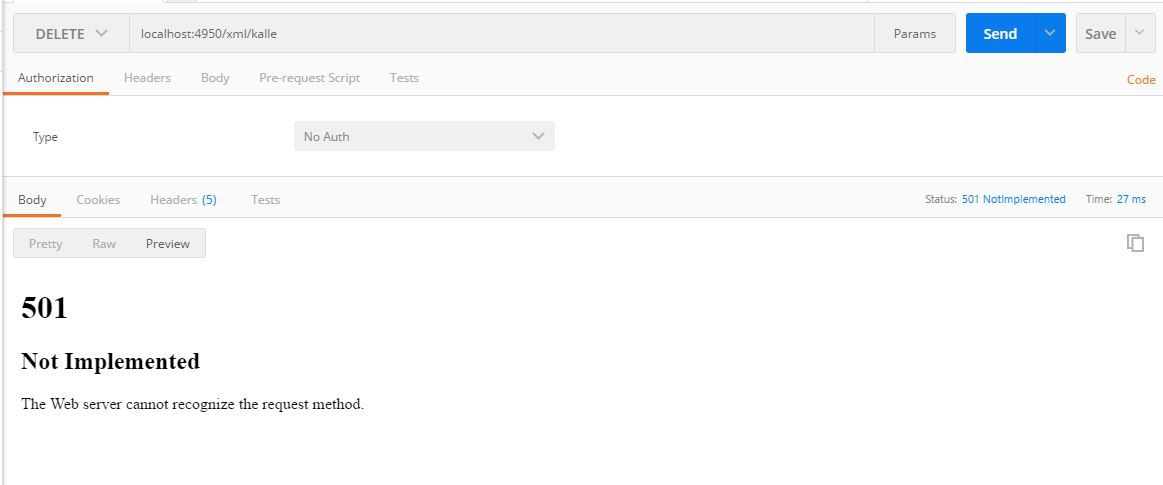
\includegraphics[width=0.95\textwidth,keepaspectratio]{img/501.jpg} 
	\caption{500 for any internal server errors, socket error etc.}
\end{figure}

\begin{figure}[h!]
	\centering
	\label{505}
	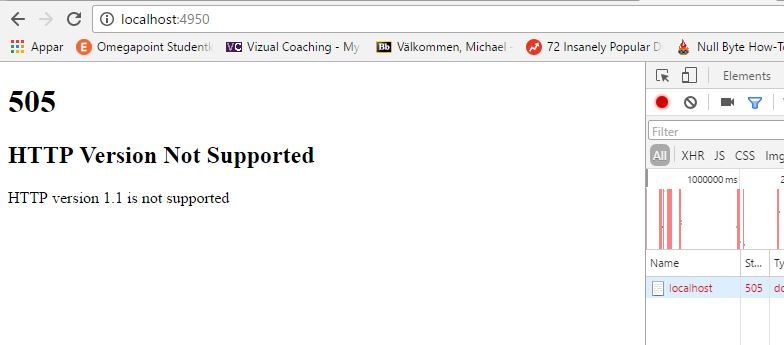
\includegraphics[width=0.95\textwidth,keepaspectratio]{img/505.jpg} 
	\caption{500 for any internal server errors, socket error etc.}
\end{figure}


\subsection{VG.2}

\end{document}
